%!TEX root = ../main.tex

\chapter{Text detection}
\label{ch:detection}

The challenges presented in \autoref{sec:challenges} make it clear that a classical approach is unsuitable for our problem. As such, we direct our attention towards the modern, robust architectures of Convolutional Neural Networks (CNN) \citep{leCun_CNN}. In particular, we take inspiration from the great advances in object detection and we will treat text like a regular object which can be found anywhere in the image.

\Autoref{sec:faster_rcnn} introduces the first architecture we tested, the \FRCNN{} \citep{faster_rcnn}, as a mean of establishing a baseline. Then we present several evaluation techniques in \autoref{sec:detection_eval} and the requirements of a good detection system. We use these to drive several experiments, which are presented in \autoref{sec:detection_experiments} together with their data; intermediate results will drive us to more advanced data generation techniques. Then, \autoref{sec:ctpn} presents a more powerful architecure for text detection, the \emph{Connectionist Text Proposal Network}(\CTPN{}, \citet{ctpn}). Finally, we conclude the chapter with an overview of the results in \autoref{sec:detection_results}.

%========================================================================================

\section{Faster R-CNN}\label{sec:faster_rcnn}

	\begin{figure}
		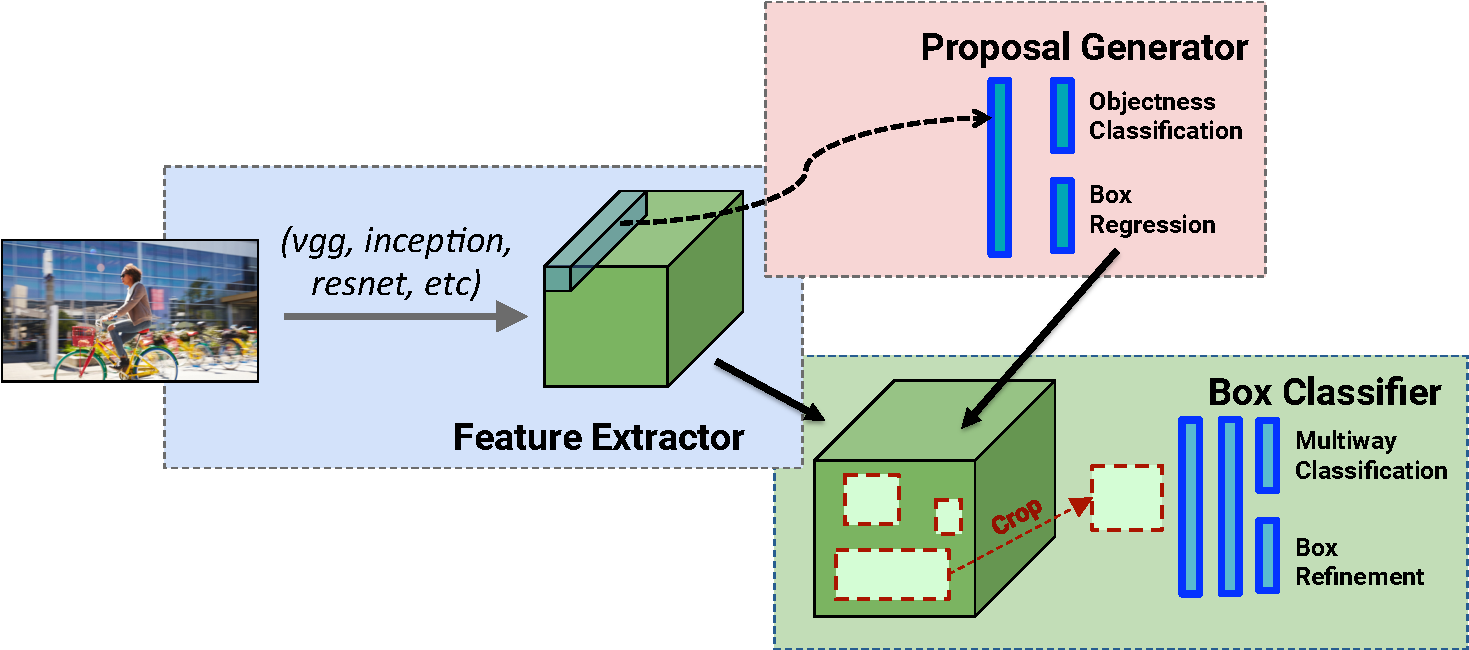
\includegraphics[width=0.85\linewidth]{fasterrcnn_diagram.pdf}
		\caption[The \FRCNN{} architecture]{(credit to \cite{detection_benchmark}) \label{fig:faster_rcnn}}
	\end{figure}

	The task of object detection builds upon that of image classification. Architectures based on region proposals (see \autoref{sec:related_detection}) can be seen as a two stage algorithm: the first part extracts possible object bounding boxes as a sub-image of the input, while the second one predicts the class associated with each candidate. It is of no surprise then that object detection greatly benefits from the super-human accuracy of deep neural networks \citep{superhuman_classif}. We chose to pair the \FRCNN{} detection architecture with the \RESNET{} feature extractor \citep{resnet}, since this has been proven as a good trade-off between detection accuracy and speed on the standard challenge of ILSCVR \citep{detection_benchmark}. In what follows we present the main building blocks of this architecture.

	%----------------------------------------------------------------------------------------

	\subsection{Feature extraction}\label{sec:resnet}
		In order to perform detection on an input image, we first need to extract representative high-level features from the raw pixel values. To this end, we employ the \RESNET{} convolutional architecture which has won many competitions in classification, detection and segmentation.

		The novelty of this approach\footnote{\todo{Should I dedicate a subsection to describe how (Conv) Neural Nets work?}} relies in forcing the network to learn a \emph{residual} mapping \(\mathcal{F}(\ve{x}) := \mathcal{H}(\ve{x}) - \ve{x}\), where \(\mathcal{H}(\ve{x})\) represents a desired mapping from input \(\ve{x}\), which is to be fit through a few stacked layers. This comes from the observation that the optimal function to be learnt could be closer to the identity mapping than to a zero mapping. Therefore, the new formulation eases the job of the optimiser since it only has to find perturbations around the identity mapping, rather than learn a completely new function.
		% http://www.robots.ox.ac.uk/~vgg/publications/2015/Jaderberg15b/jaderberg15b.pdf gives a good started about many things, including how ConvNets work

		Moreover, in order to keep the number of parameters as small as possible and have reasonable training times for very deep architectures (101 layers), standard convolutions are replaced by bottleneck-blocks of convolutions (\autoref{fig:resnet} right). Such blocks are formed by concatenating a \(1 \times 1\) convolutional layer at each end of the \(3 \times 3\) layer. The ``prefix'' layer reduces the number of filters while the ``suffix'' one increases it back, thus reducing the computational cost of the heavier middle layer.

		\begin{figure}
			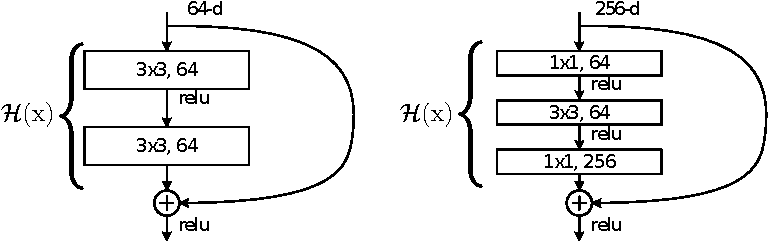
\includegraphics[width=0.85\linewidth]{resnet}
			\caption[ResNet blocks]{
				(\citet{resnet})
				\todo{Add \(\mathcal{H}(\ve{x})\) on the schema and small explanation.}
				\label{fig:resnet}
			}
		\end{figure}

		\todo{Show examples of extracted features for detection ? }

	%----------------------------------------------------------------------------------------

	\subsection{Region proposal network}\label{sec:frcnn_rpn}
		In order to bring the inference speed closer to real-time, \FRCNN{} improves on the bottleneck of previous approaches, namely the proposal of object candidates. Instead of relying on highly-engineered low-level features of super-pixels, the architecture reuses the convolutional feature map generated for the region classification step.

		This is achieved through another small, fully-convolutional network which is slided along the final layer of the feature map. The window at each location is projected into a lower dimensional feature that is used to predict \(k\) region bounds as well as \(k\) ``objectness'' scores. Each predicted region \(k_i\) is encoded as 4  coordinates \((x_1, y_1, x_2, y_2)_i\) that are \emph{relative} to a set of predefined boxes called \emph{anchors}. This mechanism allows the detection of multiple scales and aspect ratios in one pass through the network, thus avoiding the need of image pyramids and further reducing the computational cost.

		For training the RPN, the following loss function has to be minimised:
		\begin{equation}\label{eq:rpn_loss}
		L(\{p_i\}, \{t_i\}) = \frac{1}{N_{\cls}}\sum_i L_{\cls}(p_i, p^{*}_i) + \lambda\frac{1}{N_{\reg}}\sum_i  p^{*}_i L_{\reg}(t_i, t^{*}_i);
		\end{equation}
		\(p_i\) represents the probability that anchor \(i\) is an object; \(p^{*}_i\) is the label of this anchor (\(1\) when it significantly overlaps a ground-truth box) and \(t_i, t^{*}_i\) encode the anchor's and ground-truth's coordinates, respectively.

		The loss jointly minimised  the ``objectness'' classification term \(L_{\cls}\) for an anchor \(i\) in the minibatch and the bounding box regression term \(L_{\reg}\); the two are balanced by the hyperparameter \(\lambda\). The regression term is only taken into account for positive anchors (\(p^{*}_i = 1\)), which are those overlapping a ground-truth box with an Intersection-over-Union (IoU) ratio above threshold \(\tau = 0.7\).

	%----------------------------------------------------------------------------------------

	\subsection{Training}\label{sec:frcnn_train}
		In addition to the RPN, the \FRCNN{} architecture also needs to classify the generated proposals. For this, it uses the Fast R-CNN architecture and trains both of them at the same time, as shown in \autoref{fig:faster_rcnn}. The forward pass generates box proposals that the classifier considers to be fixed for its training. This easy implementation ignores the gradients with regards to the coordinates of the proposal boxes, so it is only an approximation of the joint training procedure. However, its results are close to those obtained by alternating the training of the two networks, while being significantly faster.

		Instead of training the whole architecture from scratch, we gain significant time by using transfer learning and starting with a model that performs well on the ImageNet challenge. We replace its final softmax layer so that it only predicts among our two classes of interest: \texttt{text} or \texttt{background}.

		We hypothesize that the object / not-object distinction is easier to make for text detection in white background documents than it is for an ImageNet object. Therefore, we set hyperparameter \(\lambda = 2\) in order to give preference to the localisation loss. Moreover, in order to account for text's wide aspect ratio and relatively constant height in our documents, we generate similarly wide anchors (ratios \(\{2, 4, 6, 8, 10\}\)) with a limited set of scales (heights of \(\{50, 75, 100\}\)px). This further helps the box regression part to converge.

		We use the stochastic gradient descent (SGD) optimiser with momentum, on batches of 1 input image. Note, however, that a minibatch is formed of bounding boxes, so many candidates can be generated from a single input image and a set of anchors. Several hyper-parameters control the composition of the batches:
		\begin{description}
			\item[number of proposals (\(\mathit{value} = 300\))] How many object proposals are generated in each batch.

			\item[positive to negative ratio (\(\mathit{value} = 0.5\))] For a robust classification and convergence of ``objectness'' score, it is important that examples of both positive and negative candidates are generated.

			\item[positive IoU threshold (\(\tau_{+} = 0.7\))] An anchor is considered positive when \(\mathit{overlap}(\mathit{anchor}, \mathit{truthBox}) > \tau_+\). While \(0.7\) can be considered low for text objects (see \autoref{fig:text_overlap_example}), setting this value too high in the early stages leads to a lower number of positive candidate and slows down convergence of \(L_{cls}\).

			\item[negative IoU threshold (\(\tau_{-} = 0.3\))] Similar to \(\tau_{+}\), but for marking candidates as negative examples.

			\item[NMS confidence threshold (\(\mathit{value} = 0.0\))] When a candidate has a low confidence score, we can supress it from contributing to the loss. We effectively disable this filter because we want to force the network to give high-confidence predictions, therefore it should learn from all examples.

			\item[NMS IoU threshold (\(\tau_{\textsc{nms}} = 0.7\))] When several proposals overlap each other, we should keep only one of them in order to encourage proposal's diversity. This parameter controls when we can consider that a proposal is redundant to another one, in terms of their overlap.

		\end{description}

		On every experiment we monitor the training progress by intermittently evaluating the model on a validation dataset of images from the same category. The training is stopped once there is no significant improvement for more than two epochs, despite a decreasing learning rate.


%========================================================================================

\section{Evaluation framework}\label{sec:detection_eval}
The lack of a \emph{cost} or risk associated with a false positive detection makes the assessment of an algorithm a very difficult task as it requires a trade-off between different types of errors. Standard object detection challenges such as PASCAL VOC \citep{pascal_voc} required participants to rank their results by a score, commonly referred to as \emph{confidence}. This allows the evaluation of a trade-off between false positives and false negatives by assessing the area under the precision/recall curve. To this end, the Average Precision is used:\[
	\operatorname{AP} = \frac{1}{11} \sum_{r \in [0,1]} p(r),
\] which is the mean of precisions \(p\) computed at eleven equally spaced recall values \(r \in [0,1]\).

Two essential observations need to be made. First, a great importance is given to the confidence score, since recall and precision are defined by only considering examples ranked above a given rank. Second, the measure does \emph{not} define what a positive result means. For object detection, a predicted bounding box \(B_p\) is positively mapped to \mbox{ground-truth} box \(B_{gt}\) when their overlap exceeds a given threshold \(\tau\). The overlap is defined as \[
	\iou(B_p, B_{gt}) = \frac{\mathit{area}(B_p \cap B_{gt})}{\mathit{area}(B_p \cup B_{gt})}.
\] In general, the threshold is set at \(\tau = 0.5\) and the measure is denoted by \(\AP\).

\todo{Problem: I'm using IoU in hyperparams of FRCNN, which comes before this section.}

Since text detection is a particular case of object detection, it generally subscribes to the same evaluation criteria. However, text is more than a simple object with binary presence; it consists of a sequence of characters, all of which are mandatory and of \emph{equal} importance to the meaning. This is in contrast to objects in general images such as those in the PASCAL VOC database. While these also present a hierarchical structure (e.g.\ a cat has eyes, ears, legs, tail etc.), the presence of their sub-elements is not always mandatory; on the contrary, a subset of composing elements is almost always hidden due to self occlusions. This allows some partial detections to be considered valid in the context of objects (see \autoref{fig:cindy}). Text detection cannot afford such flexibility, since we aim to use the detections in a subsequent step of transcription. This requires that bounding boxes include all relevant text and, ideally, no other text fragments such as parts of the line above or below (see \autoref{fig:text_overlap_example}).

Considering that in our documents text lines are close to each other, we demand the detections to be as tight as possible around the text. In addition, having a high recall is more important than predicting with a high confidence, since the transcription phase can easily ignore false positives. For this reason, the comparison in \autoref{sec:frcnn_results} will consider these two criteria for comparing different experiments. However, given the lack of a detection baseline in such challenging documents, we based our intermediate decisions on the standard measure of \(\AP\) which allowed us to compare with the performance of the same algorithm on a different task.

\subsubsection*{Test data}\label{sec:detection_test_data}

Given that our approaches rely on transfer learning, we need an objective way of comparing their performance. To this end, we constructed a \ds{TEST} dataset to provide ground truth labels on real-world data. This consists of 26 annotated statements which amount to approximately 1400 bounding boxes.

\begin{figure}
	\begin{subfigure}[b]{0.49\linewidth}
		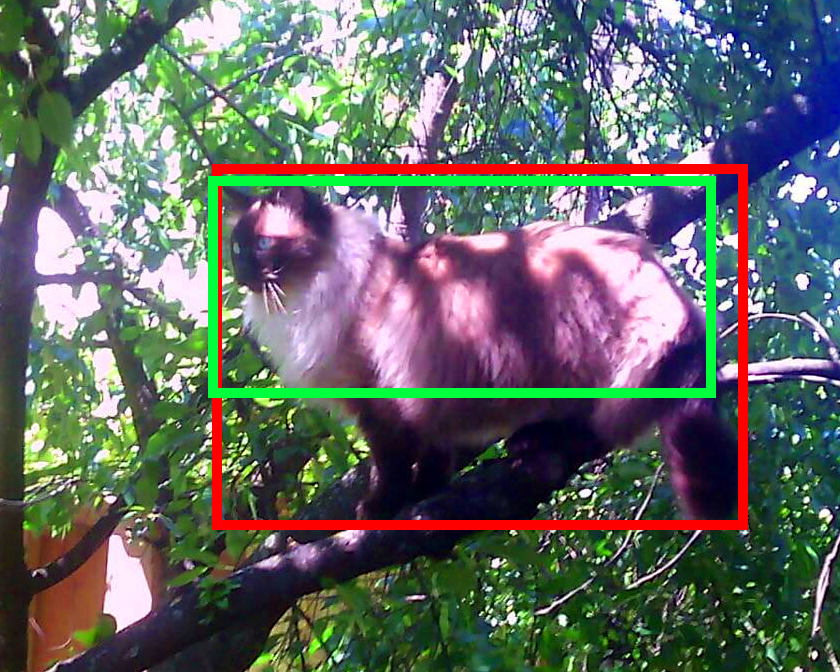
\includegraphics{cindy}
		\caption{\label{fig:cindy}}
	\end{subfigure}
	\begin{subfigure}[b]{0.49\linewidth}
		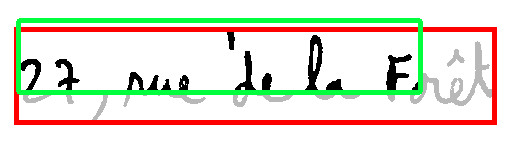
\includegraphics{text_iou}
		\vspace{2em} % no idea why this works. it was supposed to add space *between* the images, but oh well...
		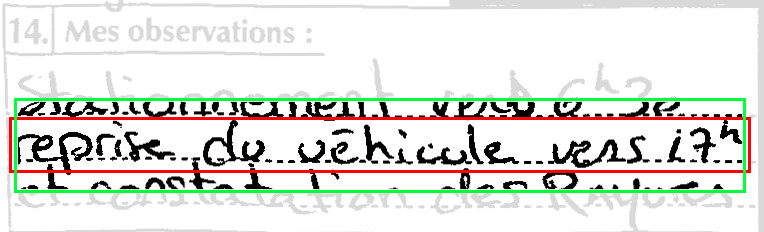
\includegraphics{text2_iou}
		\caption{\label{fig:text_overlap_example}}
	\end{subfigure}
	\caption[Overlap examples]{Overlap examples: red shows ground-truth; green shows detection. In all cases \(\iou = 0.55\). While this is a valid detection threshold for a normal object, it is unsatisfactory for text recognition.
	}
	\label{fig:overlap_example}
\end{figure}


%========================================================================================


\section{Generating data for training experiments}\label{sec:detection_experiments}
	Given the large number of parameters in deep neural networks (\(\approx 6 \times 10^8\) for \RESNET{}), it is clear that large amounts of training data are needed. Since this is lacking for our project, we must find alternative sources of handwritten text, ideally in the same language as the documents, i.e. French. Moreover, as was noted in \autoref{sec:challenges}, our documents have a specific format and less than optimal quality. The rest of the section shows how we transition from the clean and neat handwriting database to a format that helps the algorithm generalise to our use case.

	%----------------------------------------------------------------------------------------

	\subsection{The RIMES database}\label{sec:rimes}
		The RIMES database \citep{rimes} is the result of a huge data collection effort by the French ministries of defense and research, which was set up in order to create a new, consistent database of handwritten text. Its novelty was that it also included mixed pages, with handwritten and printed text, as well as being almost completely unconstrained with regards to the content of the text.	It contains more than \(50\,000\) handwritten words that are made available individually, or in lines (more than \(9000\)), or in paragraphs (more than \(1500\)).

	%----------------------------------------------------------------------------------------

	\subsection{Collage of paragraphs}
		For the first training session, we used images of paragraphs from the database along with their segmentations into lines as labels. To make them resemble the format of the documents, we juxtaposed two or three paragraphs picked at random from the database. These were corrected for rotation and augmented with borders, similarly to the sections in a document (\autoref{fig:collage}). We generated \(3500\) examples for training and \(500\) for validation. In our comparisons, we will refer to this dataset as \ds{Collage}.

		A model trained on this dataset converged rather quickly, in \(\approx 8000\) iterations. On its validation data, the model achieves a remarkably high performance, with \mbox{\(\AP = 0.96\)}. Note that the best performance of any model in object detection so far is \(\AP \simeq 0.73\), which clearly indicates that the task is very easy for the chosen model. However, the performance does not extend to the \ds{TEST} dataset, achieving only \(\AP = 0.02\). This highlights the differences between the training and the test dataset. The most likely cause of the performance drop is the presence of additional elements in a real document, such as printed text and indicator lines, which do not exist in the training images. Therefore, the negative anchors generated by the algorithm are inevitably white boxes. In addition, the model regresses the default anchor sizes to predict boxes of shape similar to the input lines. These present little variation in width and are, in general, much wider than the text fields of a document.

		\begin{figure}
			\begin{subfigure}[c]{\textwidth}
				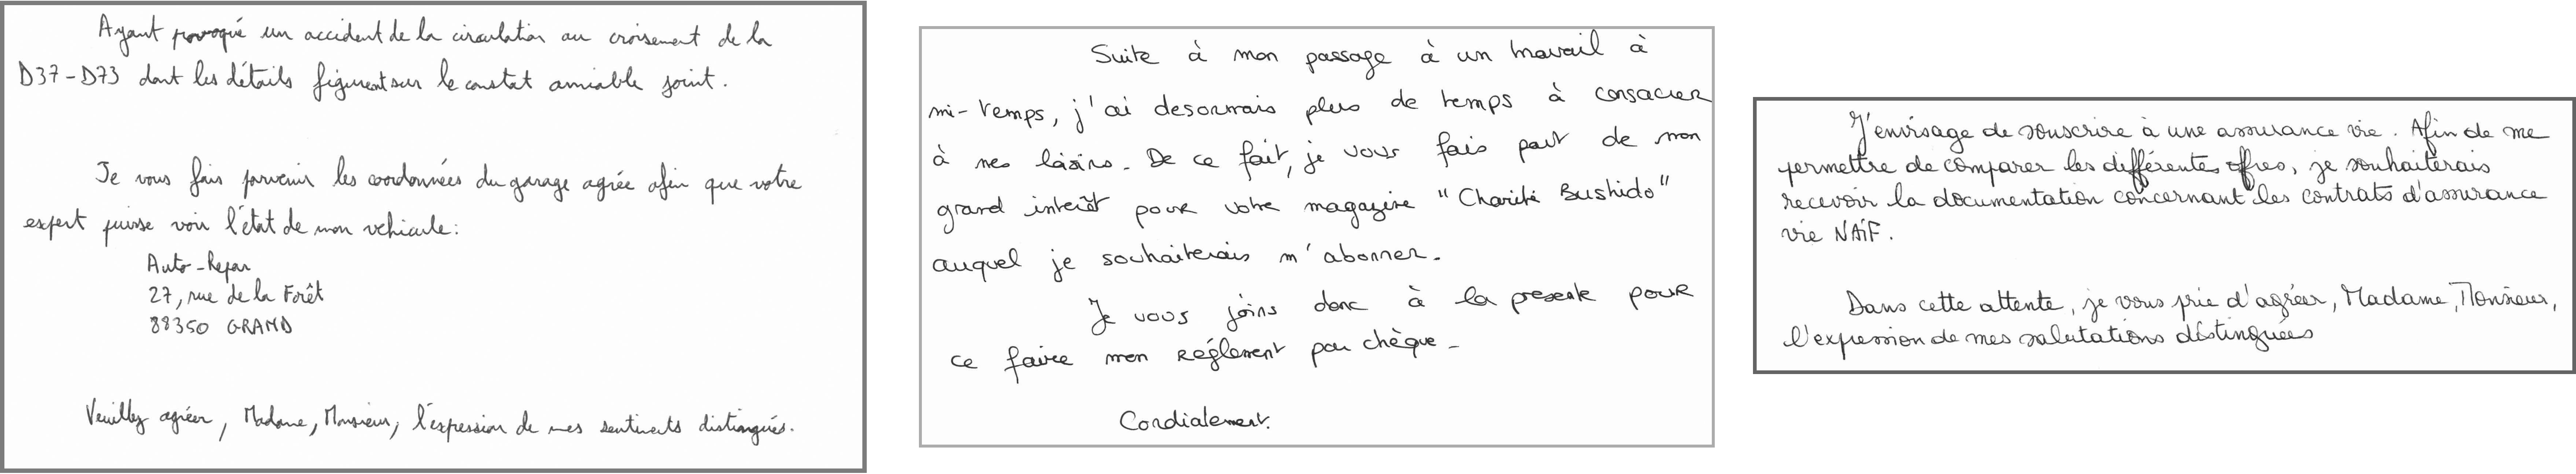
\includegraphics{collage_3}
				\caption{}
				\label{sfig:collage_clean}
			\end{subfigure}
			\vspace{1em}

			\begin{subfigure}[c]{\textwidth}
				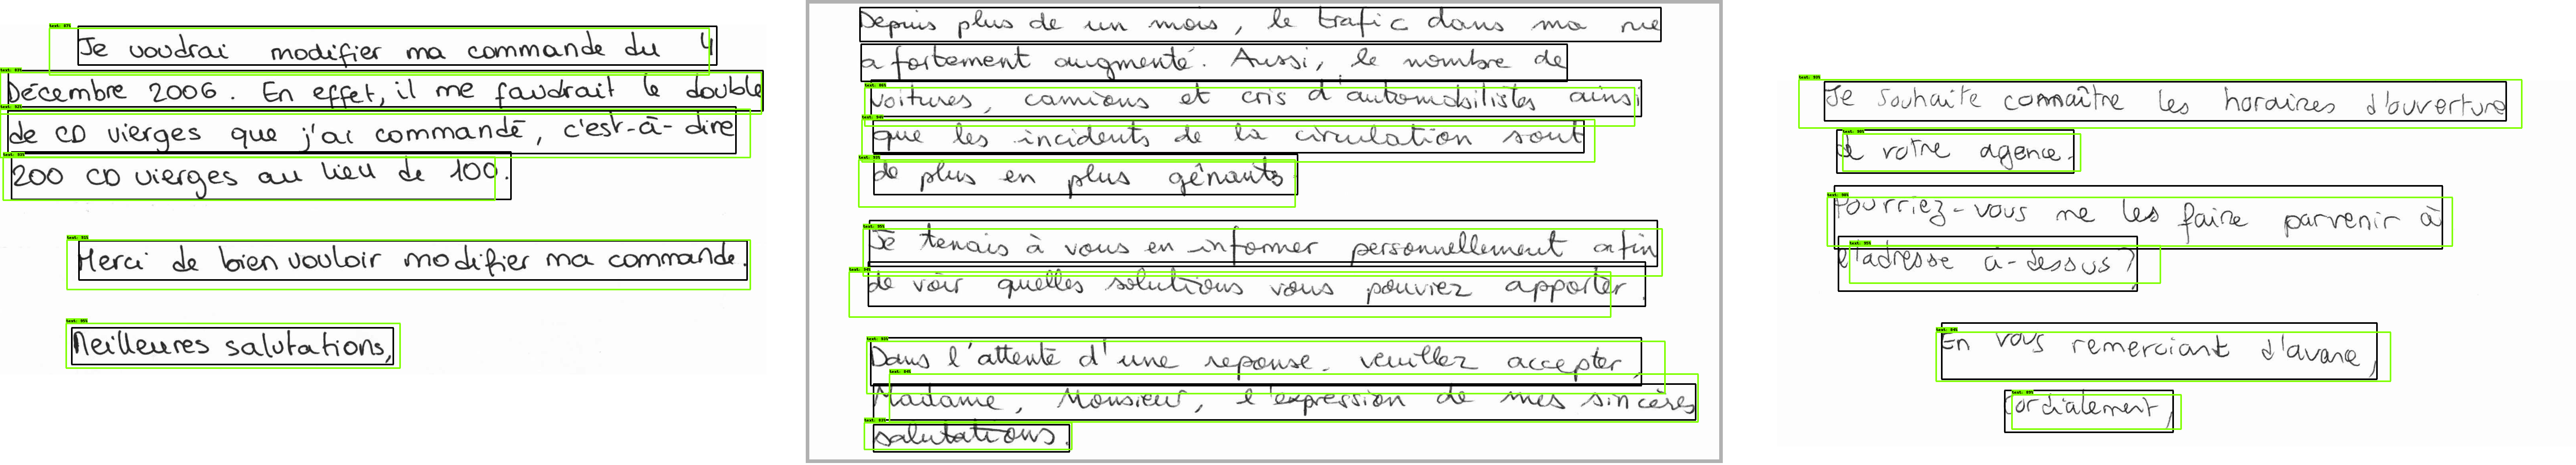
\includegraphics{collage_3_detected}
				\caption{}
				\label{sfig:collage_detect}
			\end{subfigure}
			\caption[\ds{Collage} dataset]{
				The \ds{Collage} dataset.
				\subref{sfig:collage_clean}: Example of generated collage document with 3 juxtaposed paragraphs.
				\subref{sfig:collage_detect}: The detection performed on such a document, with ground-truth in black and detection result in green.
			}
			\label{fig:collage}
		\end{figure}

	%----------------------------------------------------------------------------------------

	\subsection{Filled templates}
		%----------------------------------------------------------------------------------------
		% subsubsection: general description

			To address the limitations of the \ds{Collage} dataset and allow the model to learn more complex patterns, we propose to generate images which resemble more the real documents. To this end, we fill accident statement templates of 4 different styles with handritten text from a database. This results in realistic looking documents while saving the high cost of manual labelling.

			A template is formed by adding input placeholders to an empty document (\autoref{fig:template}). These correspond to the standard places that the users need to fill as well as non-standard places where users regularly add information. To increase the variation of the data, only a subset of the placeholders are filled on each template instance and the input text is shifted to the right of the placeholder's edge with a random amount. We investigate two possible text sources for filling the placeholder.

			The first one consists of images of \emph{individual} words from the RIMES database. This has the advantage of tight bounding boxes around the text, which we established as an important criterion (see \autoref{sec:detection_eval}). Also, it allows us to keep the ground-truth text associated with each box, which could be beneficial for the transcription step. On the other hand, this source also poses some problems. First, words are generally shorter than the placeholders, so we would need to concatenate several words to resemble the real data. Since the word order was lost when constructing the database, this has the disadvantage that the lines formed this way do not follow any sentence structure. Furthermore, words with ascenders and descenders would need to be aligned to their baseline, which is especially difficult to estimate for short words. Finally, handwriting styles from multiple authors would be combined on the same line and in the same document section.

			The second source of text consists of images of text lines from the same database. This addresses the problems of word concatenation, but introduces another difficulty: the lines usually do not fit inside the placeholders, so they need to be cut. However, thinking forward about the text transcription part, we immediately realise that in order to have reliable \((\mathtt{image}, \mathtt{label})\) pairs, we must ensure line images are split \emph{only between the words}. We use the following algorithm to detect good splitting points in image \(\ma{I}\):\footnote{\todo{use some ``algorithm'' package here; although these are quite fixed}} % https://tex.stackexchange.com/questions/172399/how-to-write-sentences-in-an-algorithm-in-latex https://tex.stackexchange.com/questions/142922/how-to-align-text-within-an-algorithm-environment
			\noindent\begin{minipage}{\linewidth}
			\begin{enumerate}
				\item use the line transcription labels to find the number of words \(n\)
				\item project the image columns horizontally, accumulating their sum into \[
					\ve{p}[c] = \sum_r \ma{I}[r,c]
				\]
				\item find the continuous runs of zero \(\ve{z} = \{ (i, j) \mid \ve{p}[k] = 0, \forall k \in [i, j] \}\); these correspond to gaps between letters (marked in red in \autoref{fig:baseline_ok})
				\item take \(n\) widest gaps \(\ve{z}'\) from \(\ve{z}\), where the gap width \(w := j - i\)
				\item split at columns \(c_k = \frac{j_k - i_k}{2}, \forall (i_k, j_k) \in \ve{z}'\).
			\end{enumerate}
			\end{minipage}
			\\

			To avoid placeholders filled with very short words, we add multiple words to the same placeholder until it is at least 75\% filled. Note that unlike the first text source, these words come in order from the original line, splitted by the above algorithm. Moreover, lines come sequentially from the same paragraph, so there is writer consistency for a good part of a template, just like in the real world.

			\begin{figure}
				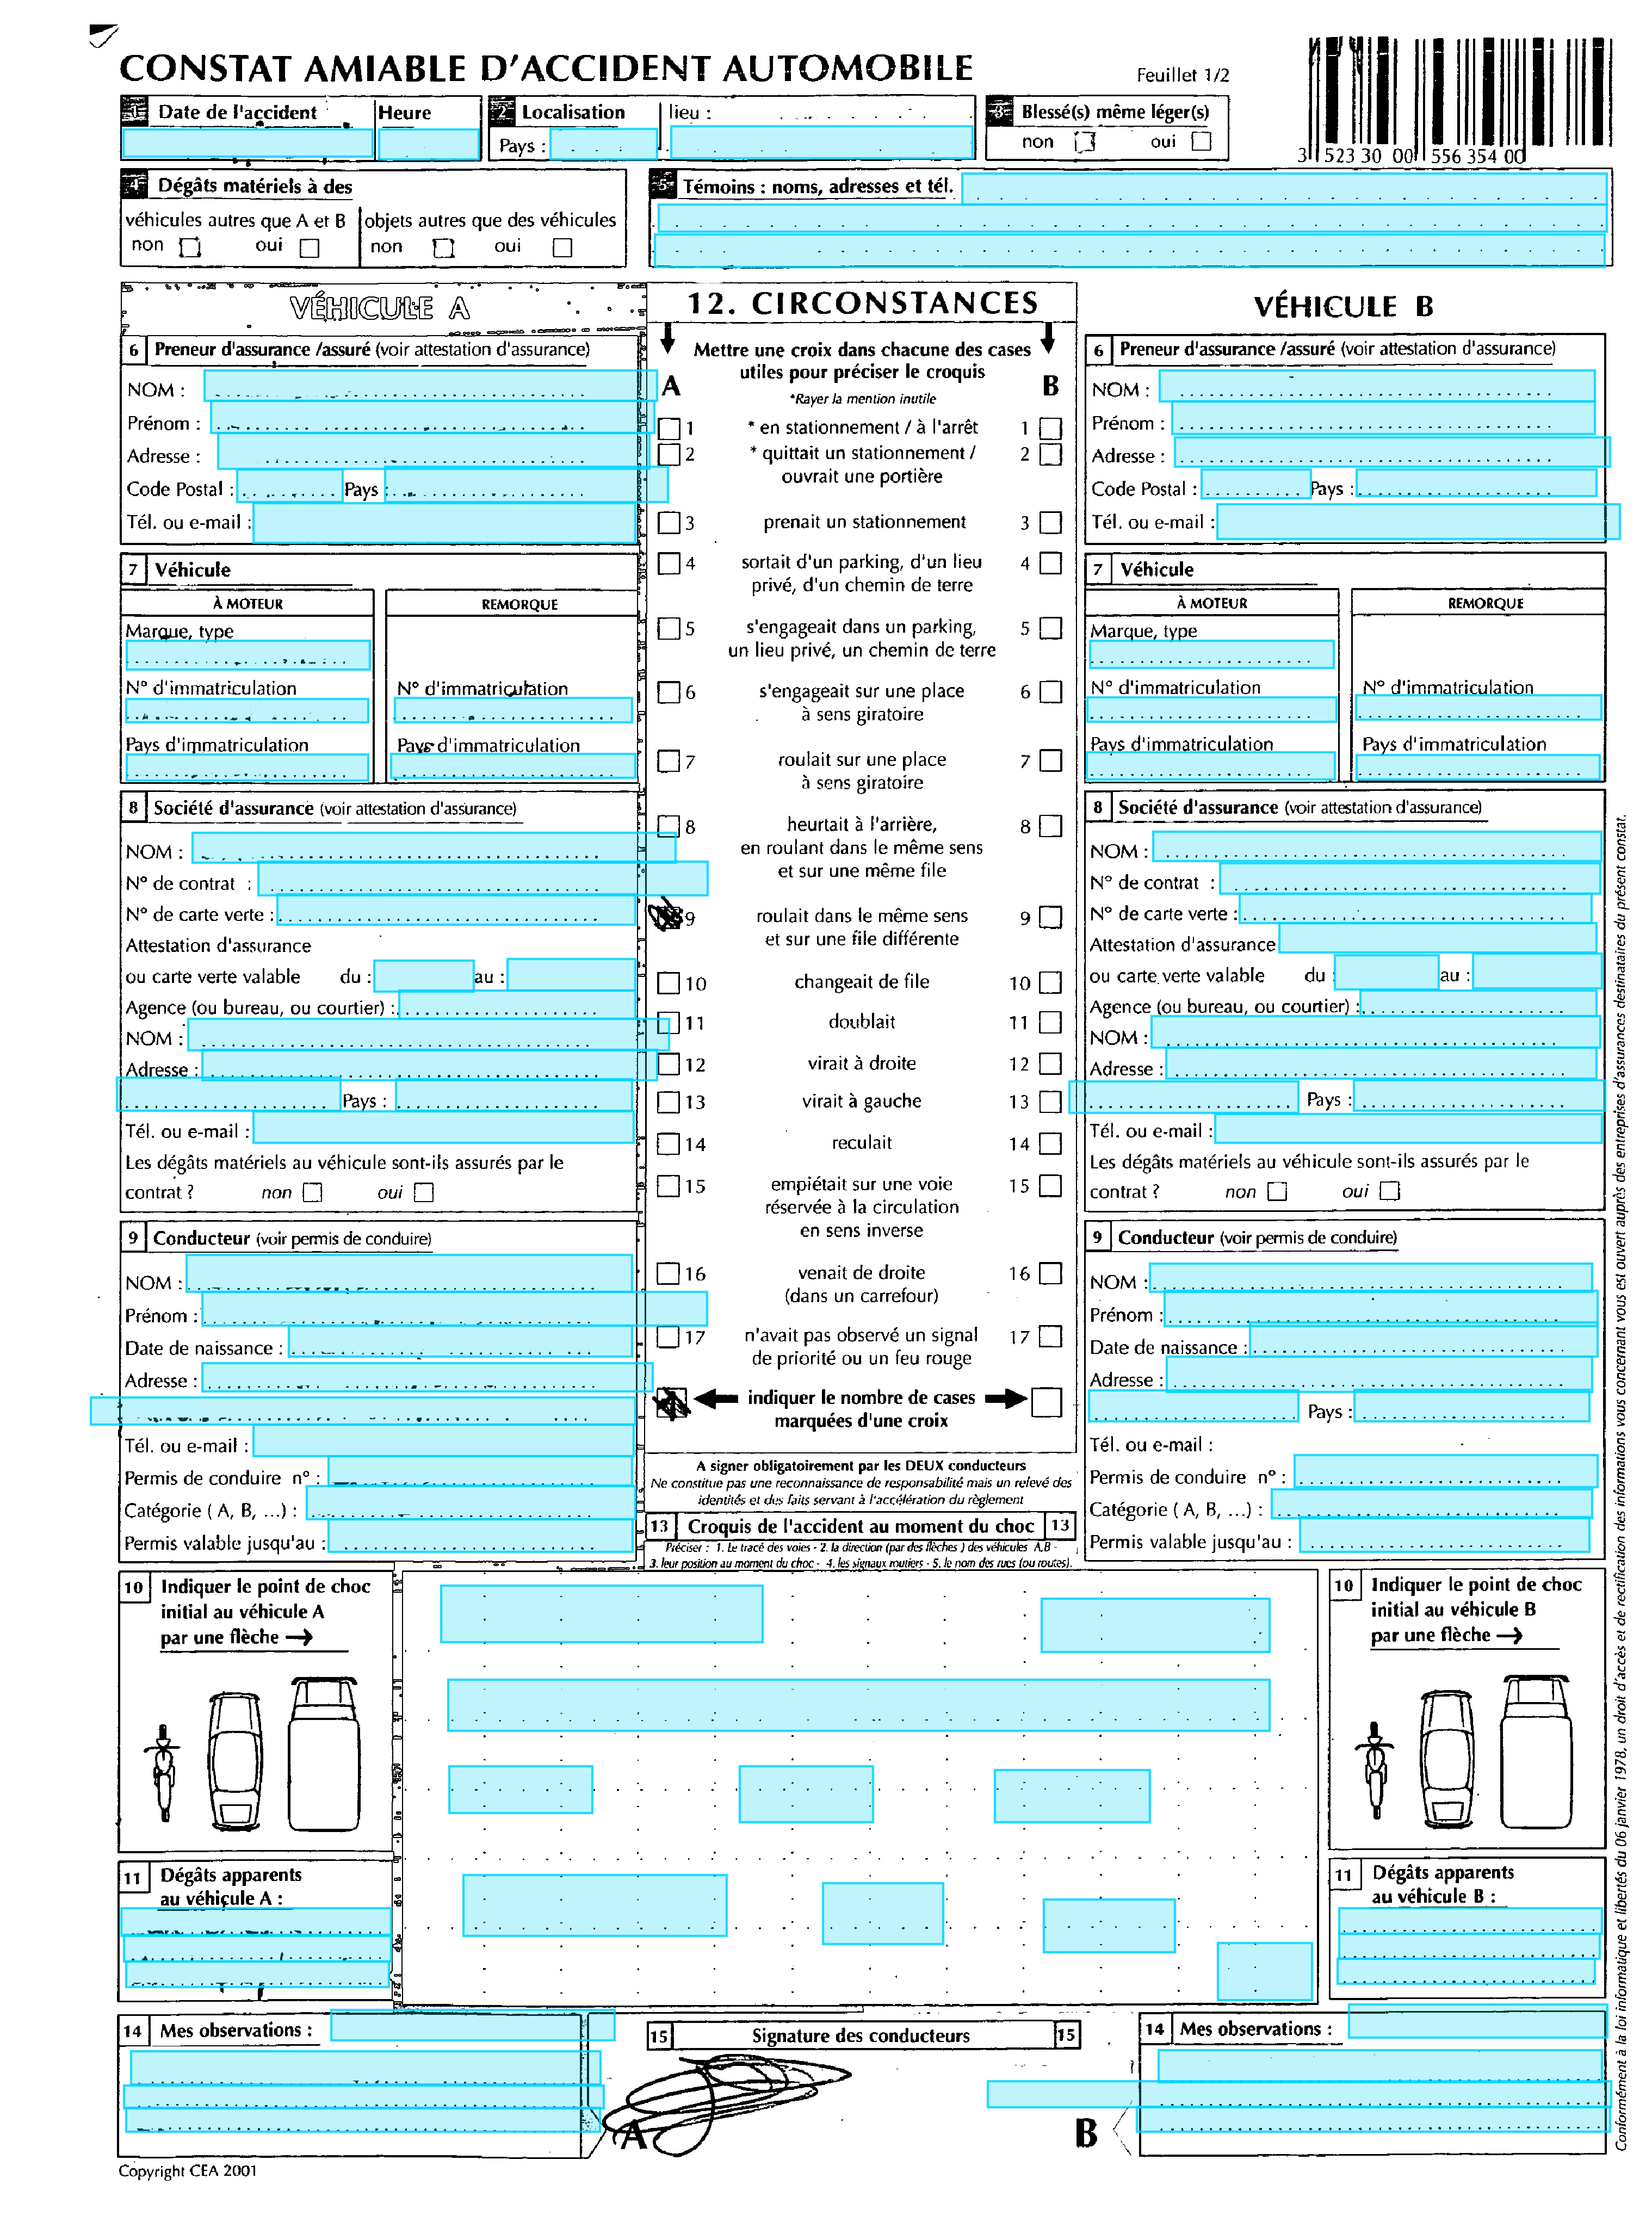
\includegraphics{template_empty}
				\caption[Document template]{An empty document template. Note that the placeholders are slightly bigger than the location for text entry in order to allow text that goes out of bounds. Also, there are placeholders in places that do not correspond to any field, which matches how people use these documents.}
				\label{fig:template}
			\end{figure}

		%----------------------------------------------------------------------------------------

		\subsubsection{Baseline detection}
			When humans fill a statement template, the baseline of their handwriting lies roughly on an indicated line.  We purposely set the placeholder's bottom edge on this line in the interest of aligning the text image in a similar manner. Then we use the following simple algorithm to find the baseline row \(r_b\) of a text image \(\ma{I}\) of size \(H \times W\) (\autoref{fig:baseline}) :
			\noindent\begin{minipage}{\linewidth}
			\begin{enumerate}
				\item project the rows of the image by averaging the pixel values: \[
					\ve{p}[r] = \frac{1}{W} \sum_c I[r,c]
				\]
				\item let \(m = \operatorname{median}(\ve{p})\)
				\item the baseline is the first row \(r_b\) where \(\ve{p}[r_b] > m\), \(b = \overline{n, 1}\).
			\end{enumerate}
			\end{minipage}\\

			This algorithm works well as long as a few assumptions hold. First, the text image has to be horizontal. In case it is not (see \autoref{fig:baseline_skewed}), we deskew it by rotating with the average angle of Hough lines. Second, the input line has to be correctly segmented vertically. As a counter example, \autoref{fig:baseline_segmentation} shows that due to another text line present in the same image it is difficult to segment the words correctly. Fortunately, the database does not contain many examples that break these assumptions and we can reject tokens resulted from a failed segmentation based on their length.

			\begin{figure}[h!]
				\begin{subfigure}{\linewidth}
					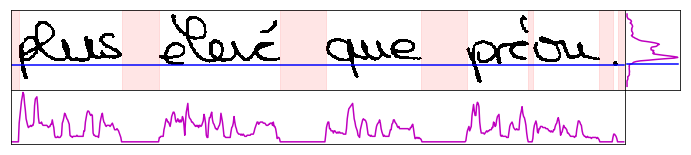
\includegraphics{baseline_ok}
					\caption{Good and clean horizontal image}
					\label{fig:baseline_ok}
				\end{subfigure}

				\begin{subfigure}{\linewidth}
					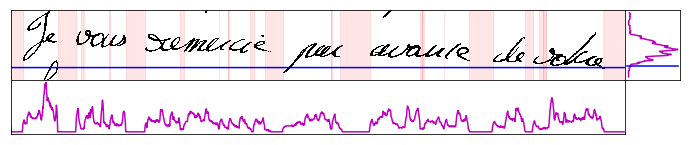
\includegraphics{baseline_skewed}
					\caption{Skewed image}
					\label{fig:baseline_skewed}
				\end{subfigure}

				\begin{subfigure}{\linewidth}
					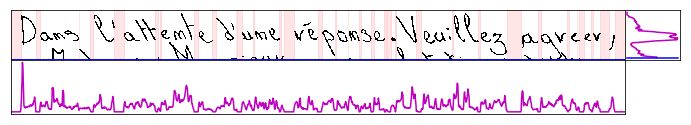
\includegraphics{baseline_segmentation}
					\caption{Badly segmented image, with slanted text}
					\label{fig:baseline_segmentation}
				\end{subfigure}
				\caption[Baseline and tokens]{Detection of the baseline and the tokens in a text image.}
				\label{fig:baseline}
			\end{figure}

		%----------------------------------------------------------------------------------------

		\subsubsection{Filling with generator}
		\startToDo
			Should we actually mention this, given that we only introduce the generator later, for transcription ?

			Also, no tests for \FRCNN{} + Generator data, only \CTPN{}. So, should I include it here or later in CTPN section ?
		\stopToDo

		%----------------------------------------------------------------------------------------

		\subsubsection{Results}
		With the above techniques we generated 2000 templates for training, for a total of 50\,000 text examples; we will refer to this dataset as \ds{Template}. It became apparent that this task was appropriately more difficult than the \ds{Collage} dataset, as the validation performance was still improving after 35\,000 steps. However, due to a slow improvement rate, we stopped the training there, as we deemed the validation performance ``good enough'' for an experiment, at \(\AP \simeq 0.76\). Surprisingly though, the perfomance on the \ds{TEST} dataset was essentially zero (\(\AP \simeq 0.007\)). A very close inspection of the generated data, in comparison to the test data, revealed a key difference between the two: the real-world documents are (almost) binarised, while the text from the RIMES database is not (\autoref{fig:template_gray_hist}). Convolutional neural networks should be robust to general appearance changes, especially when random contrast is used as a data augmentation technique. However, knowing that the first filters of CNNs correspond to edge extractors, we hypothesise that the disruption is given by the transitions from foreground (text) to background (white). In the case of RIMES, these are soft edges and only extreme contrast boosts can convert them into hard edges.

		\begin{figure}
			\begin{subfigure}{\linewidth}
				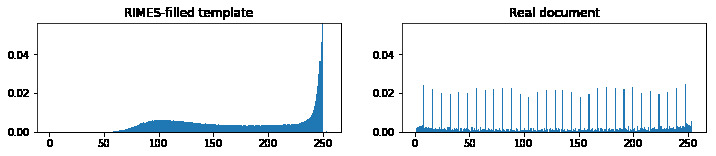
\includegraphics{template_hist}
			\end{subfigure}
			\begin{subfigure}{\linewidth}
				
\includegraphics[width=.49\linewidth]{binarisation_template}
				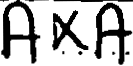
\includegraphics[width=.49\linewidth]{binarisation_real}
			\end{subfigure}
			\caption[Template histograms]{
				Top row shows normalised histograms of text-filled template and real document, with the extreme counts removed (0 and 255). The templates present more shades of gray (left) than a real document (right). Moreover, only half of real documents present such a structure, the other half being completely binarised.

				The bottom row shows examples of text from the database and from a real document. Note the soft versus hard edges.
			}
			\label{fig:template_gray_hist}
		\end{figure}

		We generated another dataset, \ds{Template_bin}, of same size as \ds{Template}, where we binarised text before pasting it into the documents. Given the uniform illumination, a global thresholding technique worked well, with the threshold chosen by Otsu's method. The model trained on this dataset converged after 4\,500 steps and has a validation \(\AP \simeq 0.83 \). It also generalizes better than previous ones on the \ds{TEST} dataset, with an \(\AP \simeq 0.37\).


	%----------------------------------------------------------------------------------------

	\subsection{Results}\label{sec:frcnn_results}

		\begin{figure}[h!]
			\begin{subfigure}{.49\linewidth}
				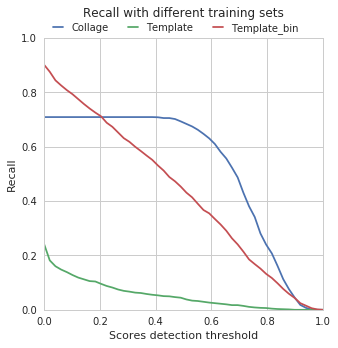
\includegraphics{frcnns_recall_scores}
				\caption{}
				\label{fig:frcnns_recall_scores}
			\end{subfigure}
			\begin{subfigure}{.49\linewidth}
				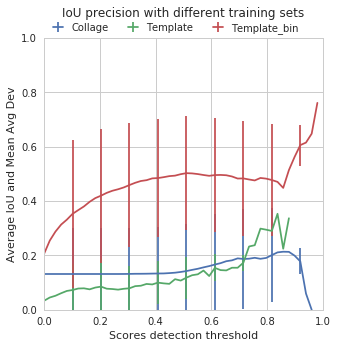
\includegraphics{frcnns_prec_scores}
				\caption{}
				\label{fig:frcnns_prec_scores}
			\end{subfigure}
			\begin{subfigure}{.49\linewidth}
				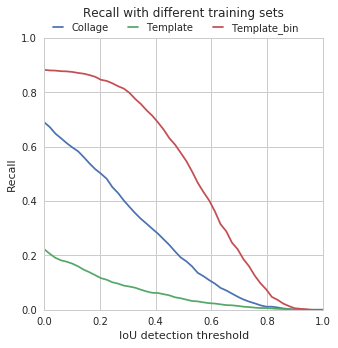
\includegraphics{frcnns_recall_iou}
				\caption{}
				\label{fig:frcnns_recall_iou}
			\end{subfigure}
			\begin{subfigure}{.49\linewidth}
				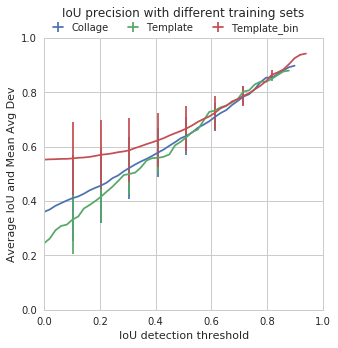
\includegraphics{frcnns_prec_iou}
				\caption{}
				\label{fig:frcnns_prec_iou}
			\end{subfigure}
			\caption[\FRCNN{} results]{\todo{...}}
			\label{fig:frcnn_results}
		\end{figure}



%========================================================================================


\section{Connectionist Text Proposal Network}\label{sec:ctpn}
	% http://i.cs.hku.hk/~kykwong/publications/wliu_bmvc16.pdf This has a good simple explanation of ResNet and LSTM and what-not


	\todo{Compare and contrast with \FRCNN{} RPN. Also, we use the VGG, because it came with the network}
%----------------------------------------------------------------------------------------


%========================================================================================


\section{Results}\label{sec:detection_results}
	This gives an overview of object detection evaluation:

	% https://www.researchgate.net/profile/Rangachar_Kasturi/publication/220928471_Performance_Evaluation_of_Object_Detection_Algorithms/links/54c91dd00cf25087c4ec62fd.pdf

	this evaluates text detection in 2 simple numbers (P, R), in terms of pixels

	http://vision.soic.indiana.edu/papers/textevaluation2000das.pdf

	\todo{Evaluation method: goal-directed approach = couple with text recognizer; see % http://citeseerx.ist.psu.edu/viewdoc/download?doi=10.1.1.332.3461&rep=rep1&type=pdf
	}
	\todo{
		Compare all \FRCNN{} with \CTPN{}
	}


%----------------------------------------------------------------------------------------
